\part{HTML Attributes}

An HTML attribute is a modifier of an HTML element. HTML attributes generally appear as name-value pairs, separated by "=", and are written within the start tag of an element, after the element's name:

\begin{lstlisting}[language=HTML]
	<tag attribute="value">(content to be modified by the tag)</tag>
\end{lstlisting}

Where tag names the HTML element, attribute is the name of the attribute, set to the provided value.

属性为 HTML 元素提供附加信息,属性应写在元素的首标签上,属性总是以名称/值对的形式出现,比如:name="value"\footnote{注意,一些元素和属性的名称采用的是美式拼写,比如color(而不是colour)。}。

属性的具体写法是:属性名称(attribute name)后紧跟一个等号(“=”),后面写上用双引号括起来的属性值(attribute value)。对于style属性的值,可以用分号(“;”)来分隔多个样式指令。


属性和属性值对大小写不敏感。不过,万维网联盟在其 HTML 4 推荐标准中推荐小写的属性/属性值,而新版本的 (X)HTML 要求使用小写属性。


The value may be enclosed in single or double quotes, although values consisting of certain characters can be left unquoted in HTML (but not XHTML). Leaving attribute values unquoted is considered unsafe.

Although most attributes are provided as paired names and values, some affect the element simply by their presence in the start tag of the element (like the ismap attribute for the img element).

不同元素使用不同的属性,属性值应该始终被包括在引号内。双引号是最常用的,不过使用单引号也没有问题。在某些个别的情况下,比如属性值本身就含有双引号,那么就必须使用单引号。

有些元素(比如body等)被添加属性的机会比较大,而有些元素(比如br等)则较小、甚至不会被添加属性。

HTML里有很多元素,同样也有很多属性。有些属性仅用于个别元素,有些属性可用于很多元素。反之亦然:有些元素只能使用个别属性,有些元素可以使用较多的属性。

\begin{table}[!h]
\centering
\begin{tabular}{|l|l|l|}
\hline
属性		&	值			& 描述	\\
\hline
class	&	\textsl{classname}	& 规定元素的类名(classname)	\\
\hline
id		& 	\textsl{id}			& 规定元素的唯一id			\\
\hline
style	& 	\textsl{style\_definiation} & 规定元素的行内样式(inline style)\\
\hline
title		& 	\textsl{text}			& 规定元素的额外信息(可在工具提示中显示)\\
\hline
\end{tabular}
\end{table}

Most elements can take any of several common attributes:

\begin{compactitem}
\item id

The id attribute provides a document-wide unique identifier for an element.[6] This can be used as CSS selector to provide presentational properties, by browsers to focus attention on the specific element, or by scripts to alter the contents or presentation of an element. Appended to the URL of the page, the URL directly targets the specific element within the document, typically a sub-section of the page. For example, the ID "Attributes" in http://en.wikipedia.org/wiki/HTML\#Attributes

\item class

The class attribute provides a way of classifying similar elements. This can be used for semantic or presentation purposes. Semantically, for example, classes are used in microformats. Presentationally, for example, an HTML document might use the designation class="notation" to indicate that all elements with this class value are subordinate to the main text of the document. Such elements might be gathered together and presented as footnotes on a page instead of appearing in the place where they occur in the HTML source.

\item style

An author may use the style non-attributal codes presentational properties to a particular element. It is considered better practice to use an element’s id or class attributes to select the element with a stylesheet, though sometimes this can be too cumbersome for a simple and specific or ad hoc application of styled properties.

\item title 

The title attribute is used to attach subtextual explanation to an element. In most browsers this attribute is displayed as what is often referred to as a tooltip.

\end{compactitem}

The abbreviation element, abbr, can be used to demonstrate these various attributes:

\begin{lstlisting}[language=HTML]
<abbr id="anId" class="aClass" style="color:blue;" title="Hypertext Markup Language">HTML</abbr>
\end{lstlisting}

This example displays as HTML; in most browsers, pointing the cursor at the abbreviation should display the title text "Hypertext Markup Language."


Most elements also take the language-related attributes lang and dir.

一般来说,一个元素包括一个首标签(start tag)、零或多个属性(attribute)、一些内容和一个尾标签(end tag),参见下图:

\begin{figure}[!h]
\centering
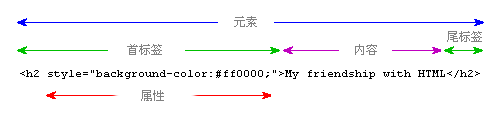
\includegraphics[scale=0.5]{htmlelements.png}
\end{figure}



\chapter{Varieties}


HTML attributes are generally classed as required attributes, optional attributes, standard attributes, and event attributes. Usually the required and optional attributes modify specific HTML elements, while the standard attributes can be applied to most HTML elements. Event attributes, added in HTML version 4, allow an element to specify scripts to be run under specific circumstances.



\section{Required and optional HTML attributes}


\subsection{Used by one tag}


\begin{compactitem}
\item <applet>: code, object
\item <area>: nohref
\item <body>: alink, background, link, text, vlink
\item <dir>: dir
\item <form>: accept-charset, action, enctype, method
\item <frame>: noresize
\item <head>: profile
\item <hr>: noshade
\item <html>: xmlns
\item <img>: ismap
\item <input>: checked, maxlength
\item <label>: for
\item <meta>: content, http-equiv, scheme
\item <object>: classid, codetag, data, declare, standby
\item <ol>: start
\item <option>: selected
\item <param>: valuetype
\item <script>: defer, xml:space
\item <select>: multiple
\item <table>: cellpadding, cellspacing, frame, rules, summary
\item <td>: headers
\end{compactitem}





\subsection{Used by two tags}

\begin{compactitem}
\item <a> and <area>:

	\begin{compactitem}
	\item coords — coordinates of an area or a link within it.
	\item shape — shape of an area or a link within it. Values: default, rect, circle, poly.
	\end{compactitem}

\item <a> and <link>:

	\begin{compactitem}
	\item hreflang — Language code of the linked document. (a, link)
	\item rel — Nature of the linked document (relative to the page currently displayed). Free text for a, but link uses a set of terms (alternate, appendix, bookmark, chapter, contents, copyright, glossary, help, home, index, next, prev, section, start, stylesheet, subsection).
	\item rev — Nature of the currently displayed page (relative to the linked document). Varies for a and link as for rel.
	\end{compactitem}

\item <applet> and <object>:

	\begin{compactitem}
	\item archive — archive URL(s) (applet, object)
	\item codebase — base URL (applet, object)
	\end{compactitem}
	
\item <basefont> and <font>:
	
	\begin{compactitem}
	\item color — text color (deprecated) (basefont, font)
	\item face — font family (deprecated) (basefont, font)
	\end{compactitem}
	
\item <col> and <colgroup>:
	
	\begin{compactitem}
	\item span — number of columns spanned (col, colgroup)
	\end{compactitem}
	
\item <del> and <ins>:
	
	\begin{compactitem}
	\item datetime — date and time of text deletion or insertion.
	\end{compactitem}
	
\item <form> and <input>:
	
	\begin{compactitem}
	\item accept — types of files accepted when uploading form or input
	\end{compactitem}
	
\item <frame> and <iframe>:
	
	\begin{compactitem}
	\item frameborder — value (0 or 1) specifies whether to display a border around the frame or iframe.
	\item marginheight — top and bottom margins in pixels around the frame or iframe.
	\item scrolling — value (yes, no, auto) specifies whether to display scroll bars around the frame or iframe.
	\item marginwidth — left and right margins in pixels around the frame or iframe.
	\end{compactitem}
	
\item <frameset> and <textarea>:
	
	\begin{compactitem}
	\item cols — number of visible columns in frameset or cols (some variation)
	\item rows — number of visible rows in frameset or rows (some variation)
	\end{compactitem}
	
\item <img> and <object>:
	
	\begin{compactitem}
	\item usemap — specifies name of a map tag to use with img -or- URL of an image-map to use with object.
	\end{compactitem}
	
\item <input> and <textarea>:

	\begin{compactitem}
	\item readonly — specifies read-only text for input and textarea.
	\end{compactitem}
	
\item <link> and <style>:

	\begin{compactitem}
	\item media — specifies display device for link and style. Values: all, aural, braille, handheld, print, projection, screen, tty, TV.
	\end{compactitem}
	
\item <optgroup> and <option>:

	\begin{compactitem}
	\item label — description text for an optgroup or option.
	\end{compactitem}
	
\item <td> and <th>:

	\begin{compactitem}
	\item abbr — abbreviated version of a table cell or header.
	\item axis — category name for a table cell or header.
	\item colspan — number of columns spanned by a table cell or header.
	\item nowrap — (deprecated) prevents wrapping of a table cell or header.
	\item rowspan — number of rows spanned by a table cell or header.
	\item scope — no effect on normal browser display, but marks a table cell or header as a logical header for other cells. Values: col, colgroup, row, rowgroup.
	\end{compactitem}
	
\end{compactitem}








\subsection{Used by multiple tags}

\begin{compactitem}
\item align — applet, col, colgroup, object, tbody, td, tfoot, th, thead, also (deprecated) in caption, div, h1 to h6, hr, iframe, img, input, legend, p, table
\item alt — applet, area, img, input
\item bgcolor — body, table, td, th, bgcolor
\item border — img, object, table
\item char — char, <colgroup>, <tbody>, <td>, <tfoot>, <th>, <thead>, <tr>
\item charoff — col, colgroup, tbody, td, tfoot, th, thead, tr
\item charset — a, link, script
\item cite — blockquote, del, ins, q
\item compact — dir, menu, ol, ul
\item disabled — button, input, optgroup, option, select, textarea
\item height - applet, iframe, img, object — also (deprecated) td, th
\item href — a, area, base, link
\item hspace — applet, object — also (deprecated) img
\item longdesc — frame, iframe, img
\item name — a, applet, button, form, frame, iframe, input, map, meta, object, param, select, textarea
\item size — basefont, font, hr, input, select
\item src — frame, iframe, img, input, script)
\item target — <a>, area, base, form, link
\item type — button, input, li, link, object, ol, param, script, style, type
\item valign — col, colgroup, tbody, td, tfoot, th, thead, tr
\item value — button, input, li, option, param
\item vspace — applet, img, object
\item width — applet, col, colgroup, hr, iframe, img, object, pre, table, td, th
\end{compactitem}







\chapter{Standard attributes}



\begin{longtable}{|l|l|l|l|l|l|l|l|l|l|}
\multicolumn{10}{r}{...}
%\tabularnewline\hline
\endhead
\hline

%\tabularnewline\hline
\endfirsthead
\multicolumn{10}{r}{...}
\endfoot
%\tabularnewline\hline
\endlastfoot
\hline
<param>		&id	    &		 &		 &		&	 &	 	&		  &			&		\\
\hline
<head>		&	    &		 &		 &		& dir & 	lang	& xml:lang & 			&		 \\
\hline
<html>		&	    &		 &		 &		& dir & 	lang	& xml:lang & 			&		 \\
\hline
<meta>		&	    &		 &		 &		& dir & 	lang	& xml:lang & 			&		 \\
\hline
<title>		&	    &		 &		 &		& dir & 	lang	& xml:lang & 			&		 \\
\hline
<style>		&	    &		 &		 &	title	& dir & 	lang	& xml:lang & 			&		 \\
\hline
<applet>		&	id &	class &	style &	title &  	 & 		& 	 	   & 			&		 \\
\hline
<br>			&	id &	class &	style &	title &  	 & 		& 	 	   & 			&		 \\
\hline
<frame>		&	id &	class &	style &	title &  	 & 		& 	 	   & 			&		 \\
\hline
<frameset>	&	id &	class &	style &	title &  	 & 		& 	 	   & 			&		 \\
\hline
<iframe>		&	id &	class &	style &	title &  	 & 		& 	 	   & 			&		 \\
\hline
<basefont>	&	id &	class &	style &	title & dir & 	lang	& 	 & 			&		 \\
\hline
<center>		&	id &	class &	style &	title & dir & 	lang	& 	 & 			&		 \\
\hline
<dir>		&	id &	class &	style &	title & dir & 	lang	& 	 & 			&		 \\
\hline
<font>		&	id &	class &	style &	title & dir & 	lang	& 	 & 			&		 \\
\hline
<menu>		&	id &	class &	style &	title & dir & 	lang	& 	 & 			&		 \\
\hline
<s>			&	id &	class &	style &	title & dir & 	lang	& 	 & 			&		 \\
\hline
<strike>		&	id &	class &	style &	title & dir & 	lang	& 	 & 			&		 \\
\hline
<u>			&	id &	class &	style &	title & dir & 	lang	& 	 & 			&		 \\
\hline
<abbr>		&	id &	class &	style &	title & dir & 	lang	& xml:lang & 			&		 \\
\hline
<acronym>	&	id &	class &	style &	title & dir & 	lang	& xml:lang & 			&		 \\
\hline
<address>	&	id &	class &	style &	title & dir & 	lang	& xml:lang & 			&		 \\
\hline
<b>			&	id &	class &	style &	title & dir & 	lang	& xml:lang & 			&		 \\
\hline
<big>		&	id &	class &	style &	title & dir & 	lang	& xml:lang & 			&		 \\
\hline
<blockquote>	&	id &	class &	style &	title & dir & 	lang	& xml:lang & 			&		 \\
\hline
<body>		&	id &	class &	style &	title & dir & 	lang	& xml:lang & 			&		 \\
\hline
<caption>		&	id &	class &	style &	title & dir & 	lang	& xml:lang & 			&		 \\
\hline
<cite>		&	id &	class &	style &	title & dir & 	lang	& xml:lang & 			&		 \\
\hline
<code>		&	id &	class &	style &	title & dir & 	lang	& xml:lang & 			&		 \\
\hline
<col>		&	id &	class &	style &	title & dir & 	lang	& xml:lang & 			&		 \\
\hline
<colgroup>	&	id &	class &	style &	title & dir & 	lang	& xml:lang & 			&		 \\
\hline
<dd>		&	id &	class &	style &	title & dir & 	lang	& xml:lang & 			&		 \\
\hline
<del>		&	id &	class &	style &	title & dir & 	lang	& xml:lang & 			&		 \\
\hline
<dfn>		&	id &	class &	style &	title & dir & 	lang	& xml:lang & 			&		 \\
\hline
<div>		&	id &	class &	style &	title & dir & 	lang	& xml:lang & 			&		 \\
\hline
<dl>			&	id &	class &	style &	title & dir & 	lang	& xml:lang & 			&		 \\
\hline
<dt>			&	id &	class &	style &	title & dir & 	lang	& xml:lang & 			&		 \\
\hline
<em>		&	id &	class &	style &	title & dir & 	lang	& xml:lang & 			&		 \\
\hline
<fieldset>	&	id &	class &	style &	title & dir & 	lang	& xml:lang & 			&		 \\
\hline
<form>		&	id &	class &	style &	title & dir & 	lang	& xml:lang & 			&		 \\
\hline
<hn>		&	id &	class &	style &	title & dir & 	lang	& xml:lang & 			&		 \\
\hline
<h1> to <h6>	&	id &	class &	style &	title & dir & 	lang	& xml:lang & 			&		 \\
\hline
<i>			&	id &	class &	style &	title & dir & 	lang	& xml:lang & 			&		 \\
\hline
<img>		&	id &	class &	style &	title & dir & 	lang	& xml:lang & 			&		 \\
\hline
<ins>		&	id &	class &	style &	title & dir & 	lang	& xml:lang & 			&		 \\
\hline
<kbd>		&	id &	class &	style &	title & dir & 	lang	& xml:lang & 			&		 \\
\hline
<li>			&	id &	class &	style &	title & dir & 	lang	& xml:lang & 			&		 \\
\hline
<link>		&	id &	class &	style &	title & dir & 	lang	& xml:lang & 			&		 \\
\hline
<map>		&	id &	class &	style &	title & dir & 	lang	& xml:lang & 			&		 \\
\hline
<noframes>	&	id &	class &	style &	title & dir & 	lang	& xml:lang & 			&		 \\
\hline
<noscript>	&	id &	class &	style &	title & dir & 	lang	& xml:lang & 			&		 \\
\hline
<ol>			&	id &	class &	style &	title & dir & 	lang	& xml:lang & 			&		 \\
\hline
<optgroup>	&	id &	class &	style &	title & dir & 	lang	& xml:lang & 			&		 \\
\hline
<option>		&	id &	class &	style &	title & dir & 	lang	& xml:lang & 			&		 \\
\hline
<p>			&	id &	class &	style &	title & dir & 	lang	& xml:lang & 			&		 \\
\hline
<pre>		&	id &	class &	style &	title & dir & 	lang	& xml:lang & 			&		 \\
\hline
<q>			&	id &	class &	style &	title & dir & 	lang	& xml:lang & 			&		 \\
\hline
<samp>		&	id &	class &	style &	title & dir & 	lang	& xml:lang & 			&		 \\
\hline
<small>		&	id &	class &	style &	title & dir & 	lang	& xml:lang & 			&		 \\
\hline
<span>		&	id &	class &	style &	title & dir & 	lang	& xml:lang & 			&		 \\
\hline
<strong>		&	id &	class &	style &	title & dir & 	lang	& xml:lang & 			&		 \\
\hline
<sub>		&	id &	class &	style &	title & dir & 	lang	& xml:lang & 			&		 \\
\hline
<sup>		&	id &	class &	style &	title & dir & 	lang	& xml:lang & 			&		 \\
\hline
<table>		&	id &	class &	style &	title & dir & 	lang	& xml:lang & 			&		 \\
\hline
<tbody>		&	id &	class &	style &	title & dir & 	lang	& xml:lang & 			&		 \\
\hline
<td>			&	id &	class &	style &	title & dir & 	lang	& xml:lang & 			&		 \\
\hline
<tfoot>		&	id &	class &	style &	title & dir & 	lang	& xml:lang & 			&		 \\
\hline
<th>			&	id &	class &	style &	title & dir & 	lang	& xml:lang & 			&		 \\
\hline
<thead>		&	id &	class &	style &	title & dir & 	lang	& xml:lang & 			&		 \\
\hline
<tr>			&	id &	class &	style &	title & dir & 	lang	& xml:lang & 			&		 \\
\hline
<tt>	          	&	id &	class &	style &	title & dir & 	lang	& xml:lang & 			&		 \\
\hline
<ul>            	&	id &	class &	style &	title & dir & 	lang	& xml:lang & 			&		 \\
\hline
<var>	   	&	id &	class &	style &	title & dir & 	lang	& xml:lang & 			&		 \\
\hline
<label>	   	&	id &	class &	style &	title & dir & 	lang	& xml:lang & accesskey &  		  \\
\hline
<legend>	   	&	id &	class &	style &	title & dir & 	lang	& xml:lang & accesskey & 		  \\
\hline
<object>	   	&	id &	class &	style &	title & dir & 	lang	& xml:lang & 			& tabindex \\
\hline
<select>	   	&	id &	class &	style &	title & dir & 	lang	& xml:lang & 			& tabindex \\
\hline
<a>	           	&	id &	class &	style &	title & dir & 	lang	& xml:lang & accesskey & tabindex \\
\hline
<area>	   	&	id &	class &	style &	title & dir & 	lang	& xml:lang & accesskey & tabindex \\
\hline
<button>	   	&	id &	class &	style &	title & dir & 	lang	& xml:lang & accesskey & tabindex \\
\hline
<input>	   	&	id &	class &	style &	title & dir & 	lang	& xml:lang & accesskey & tabindex \\
\hline
<textarea> 	&	id &	class &	style &	title & dir & 	lang	& xml:lang & accesskey & tabindex \\
\hline
\end{longtable}






\section{Event attributes}


\zihao{8}

%\begin{sidewaystable}{!h}
\begin{longtable}{|p{18pt}|p{15pt}|p{15pt}|p{10pt}|p{16pt}|p{16pt}|p{16pt}|p{16pt}|p{16pt}|p{16pt}|p{16pt}|p{16pt}|p{16pt}|p{16pt}|p{16pt}|p{16pt}|p{16pt}|p{16pt}|}
\multicolumn{18}{r}{...}
%\tabularnewline\hline
\endhead
\hline

%\tabularnewline\hline
\endfirsthead
\multicolumn{18}{r}{...}
\endfoot
%\tabularnewline\hline
\endlastfoot
\hline
<frameset>	& onload	& onunload &	&& 		&  &  &  &  &  &  &  &  &  & & & \\				
\hline													
<body>		& onload	& onunload &	&onclick	& ondblclick & onmousedown & onmousemove & onmouseout & onmouseover & onmouseup & onkeydown & onkeypress & onkeyup & & & & \\ 		
\hline
<abbr>		&	&	&	& onclick	& ondblclick & onmousedown & onmousemove & onmouseout & onmouseover & onmouseup & onkeydown & onkeypress & onkeyup & & & & \\				
\hline
<acronym>	&	&	&	& onclick	& ondblclick & onmousedown & onmousemove & onmouseout & onmouseover & onmouseup & onkeydown & onkeypress & onkeyup & & & & \\				
\hline
<address>	&	&	&	& onclick	& ondblclick & onmousedown & onmousemove & onmouseout & onmouseover & onmouseup & onkeydown & onkeypress & onkeyup & & & & \\				
\hline
<b>			&	&	&	& onclick	& ondblclick & onmousedown & onmousemove & onmouseout & onmouseover & onmouseup & onkeydown & onkeypress & onkeyup & & & & \\
\hline
<big>		&	&	&	& onclick	& ondblclick & onmousedown & onmousemove & onmouseout & onmouseover & onmouseup & onkeydown & onkeypress & onkeyup & & & & \\
\hline
<blockquote>	&	&	&	& onclick	& ondblclick & onmousedown & onmousemove & onmouseout & onmouseover & onmouseup & onkeydown & onkeypress & onkeyup & & & & \\
\hline
<caption>		&	&	&	& onclick	& ondblclick & onmousedown & onmousemove & onmouseout & onmouseover & onmouseup & onkeydown & onkeypress & onkeyup & & & & \\
\hline
<center>		&	&	&	& onclick	& ondblclick & onmousedown & onmousemove & onmouseout & onmouseover & onmouseup & onkeydown & onkeypress & onkeyup & & & & \\
\hline
<cite>		&	&	&	& onclick	& ondblclick & onmousedown & onmousemove & onmouseout & onmouseover & onmouseup & onkeydown & onkeypress & onkeyup & & & & \\
\hline
<code>		&	&	&	& onclick	& ondblclick & onmousedown & onmousemove & onmouseout & onmouseover & onmouseup & onkeydown & onkeypress & onkeyup & & & & \\
\hline
<col>		&	&	&	& onclick	& ondblclick & onmousedown & onmousemove & onmouseout & onmouseover & onmouseup & onkeydown & onkeypress & onkeyup & & & & \\
\hline
<colgroup>	&	&	&	& onclick	& ondblclick & onmousedown & onmousemove & onmouseout & onmouseover & onmouseup & onkeydown & onkeypress & onkeyup & & & & \\
\hline
<dd>		&	&	&	& onclick	& ondblclick & onmousedown & onmousemove & onmouseout & onmouseover & onmouseup & onkeydown & onkeypress & onkeyup & & & & \\
\hline
<del>		&	&	&	& onclick	& ondblclick & onmousedown & onmousemove & onmouseout & onmouseover & onmouseup & onkeydown & onkeypress & onkeyup & & & & \\
\hline
<dfn>		&	&	&	& onclick	& ondblclick & onmousedown & onmousemove & onmouseout & onmouseover & onmouseup & onkeydown & onkeypress & onkeyup & & & & \\
\hline
<dir>		&	&	&	& onclick	& ondblclick & onmousedown & onmousemove & onmouseout & onmouseover & onmouseup & onkeydown & onkeypress & onkeyup & & & & \\
\hline
<div>		&	&	&	& onclick	& ondblclick & onmousedown & onmousemove & onmouseout & onmouseover & onmouseup & onkeydown & onkeypress & onkeyup & & & & \\
\hline
<dl>			&	&	&	& onclick	& ondblclick & onmousedown & onmousemove & onmouseout & onmouseover & onmouseup & onkeydown & onkeypress & onkeyup & & & & \\
\hline
<dt>			&	&	&	& onclick	& ondblclick & onmousedown & onmousemove & onmouseout & onmouseover & onmouseup & onkeydown & onkeypress & onkeyup & & & & \\
\hline
<em>		&	&	&	& onclick	& ondblclick & onmousedown & onmousemove & onmouseout & onmouseover & onmouseup & onkeydown & onkeypress & onkeyup & & & & \\
\hline
<fieldset>	&	&	&	& onclick	& ondblclick & onmousedown & onmousemove & onmouseout & onmouseover & onmouseup & onkeydown & onkeypress & onkeyup & & & & \\
\hline
<h1>to<h6>	&	&	&	& onclick	& ondblclick & onmousedown & onmousemove & onmouseout & onmouseover & onmouseup & onkeydown & onkeypress & onkeyup & & & & \\
\hline
<hr>			&	&	&	& onclick	& ondblclick & onmousedown & onmousemove & onmouseout & onmouseover & onmouseup & onkeydown & onkeypress & onkeyup & & & & \\
\hline
<i>			&	&	&	& onclick	& ondblclick & onmousedown & onmousemove & onmouseout & onmouseover & onmouseup & onkeydown & onkeypress & onkeyup & & & & \\
\hline
<ins>		&	&	&	& onclick	& ondblclick & onmousedown & onmousemove & onmouseout & onmouseover & onmouseup & onkeydown & onkeypress & onkeyup & & & & \\
\hline
<kbd>		&	&	&	& onclick	& ondblclick & onmousedown & onmousemove & onmouseout & onmouseover & onmouseup & onkeydown & onkeypress & onkeyup & & & & \\
\hline
<legend>		&	&	&	& onclick	& ondblclick & onmousedown & onmousemove & onmouseout & onmouseover & onmouseup & onkeydown & onkeypress & onkeyup & & & & \\
\hline
<li>			&	&	&	& onclick	& ondblclick & onmousedown & onmousemove & onmouseout & onmouseover & onmouseup & onkeydown & onkeypress & onkeyup & & & & \\
\hline
<link>		&	&	&	& onclick	& ondblclick & onmousedown & onmousemove & onmouseout & onmouseover & onmouseup & onkeydown & onkeypress & onkeyup & & & & \\
\hline
<map>		&	&	&	& onclick	& ondblclick & onmousedown & onmousemove & onmouseout & onmouseover & onmouseup & onkeydown & onkeypress & onkeyup & & & & \\
\hline
<menu>		&	&	&	& onclick	& ondblclick & onmousedown & onmousemove & onmouseout & onmouseover & onmouseup & onkeydown & onkeypress & onkeyup & & & & \\
\hline
<noframes>	&	&	&	& onclick	& ondblclick & onmousedown & onmousemove & onmouseout & onmouseover & onmouseup & onkeydown & onkeypress & onkeyup & & & & \\
\hline
<noscript>	&	&	&	& onclick	& ondblclick & onmousedown & onmousemove & onmouseout & onmouseover & onmouseup & onkeydown & onkeypress & onkeyup & & & & \\
\hline
<ol>			&	&	&	& onclick	& ondblclick & onmousedown & onmousemove & onmouseout & onmouseover & onmouseup & onkeydown & onkeypress & onkeyup & & & & \\
\hline
<optgroup>	&	&	&	& onclick	& ondblclick & onmousedown & onmousemove & onmouseout & onmouseover & onmouseup & onkeydown & onkeypress & onkeyup & & & & \\
\hline
<option>		&	&	&	& onclick	& ondblclick & onmousedown & onmousemove & onmouseout & onmouseover & onmouseup & onkeydown & onkeypress & onkeyup & & & & \\
\hline
<p>			&	&	&	& onclick	& ondblclick & onmousedown & onmousemove & onmouseout & onmouseover & onmouseup & onkeydown & onkeypress & onkeyup & & & & \\
\hline
<pre>		&	&	&	& onclick	& ondblclick & onmousedown & onmousemove & onmouseout & onmouseover & onmouseup & onkeydown & onkeypress & onkeyup & & & & \\
\hline
<q>			&	&	&	& onclick	& ondblclick & onmousedown & onmousemove & onmouseout & onmouseover & onmouseup & onkeydown & onkeypress & onkeyup & & & & \\
\hline
<s>			&	&	&	& onclick	& ondblclick & onmousedown & onmousemove & onmouseout & onmouseover & onmouseup & onkeydown & onkeypress & onkeyup & & & & \\
\hline
<samp>		&	&	&	& onclick	& ondblclick & onmousedown & onmousemove & onmouseout & onmouseover & onmouseup & onkeydown & onkeypress & onkeyup & & & & \\
\hline
<small>		&	&	&	& onclick	& ondblclick & onmousedown & onmousemove & onmouseout & onmouseover & onmouseup & onkeydown & onkeypress & onkeyup & & & & \\
\hline
<span>		&	&	&	& onclick	& ondblclick & onmousedown & onmousemove & onmouseout & onmouseover & onmouseup & onkeydown & onkeypress & onkeyup & & & & \\
\hline
<strike>		&	&	&	& onclick	& ondblclick & onmousedown & onmousemove & onmouseout & onmouseover & onmouseup & onkeydown & onkeypress & onkeyup & & & & \\
\hline
<strong>		&	&	&	& onclick	& ondblclick & onmousedown & onmousemove & onmouseout & onmouseover & onmouseup & onkeydown & onkeypress & onkeyup & & & & \\
\hline
<sub>		&	&	&	& onclick	& ondblclick & onmousedown & onmousemove & onmouseout & onmouseover & onmouseup & onkeydown & onkeypress & onkeyup & & & & \\
\hline
<sup>		&	&	&	& onclick	& ondblclick & onmousedown & onmousemove & onmouseout & onmouseover & onmouseup & onkeydown & onkeypress & onkeyup & & & & \\
\hline
<table>		&	&	&	& onclick	& ondblclick & onmousedown & onmousemove & onmouseout & onmouseover & onmouseup & onkeydown & onkeypress & onkeyup & & & & \\
\hline
<tbody>		&	&	&	& onclick	& ondblclick & onmousedown & onmousemove & onmouseout & onmouseover & onmouseup & onkeydown & onkeypress & onkeyup & & & & \\
\hline
<td>			&	&	&	& onclick	& ondblclick & onmousedown & onmousemove & onmouseout & onmouseover & onmouseup & onkeydown & onkeypress & onkeyup & & & & \\
\hline
<tfoot>		&	&	&	& onclick	& ondblclick & onmousedown & onmousemove & onmouseout & onmouseover & onmouseup & onkeydown & onkeypress & onkeyup & & & & \\
\hline
<th>			&	&	&	& onclick	& ondblclick & onmousedown & onmousemove & onmouseout & onmouseover & onmouseup & onkeydown & onkeypress & onkeyup & & & & \\
\hline
<thead>		&	&	&	& onclick	& ondblclick & onmousedown & onmousemove & onmouseout & onmouseover & onmouseup & onkeydown & onkeypress & onkeyup & & & & \\
\hline
<tr>			&	&	&	& onclick	& ondblclick & onmousedown & onmousemove & onmouseout & onmouseover & onmouseup & onkeydown & onkeypress & onkeyup & & & & \\
\hline
<tt>			&	&	&	& onclick	& ondblclick & onmousedown & onmousemove & onmouseout & onmouseover & onmouseup & onkeydown & onkeypress & onkeyup & & & & \\
\hline
<u>			&	&	&	& onclick	& ondblclick & onmousedown & onmousemove & onmouseout & onmouseover & onmouseup & onkeydown & onkeypress & onkeyup & & & & \\
\hline
<ul>			&	&	&	& onclick	& ondblclick & onmousedown & onmousemove & onmouseout & onmouseover & onmouseup & onkeydown & onkeypress & onkeyup & & & & \\
\hline
<var>		&	&	&	& onclick	& ondblclick & onmousedown & onmousemove & onmouseout & onmouseover & onmouseup & onkeydown & onkeypress & onkeyup & & & & \\
\hline
<img>		&	&	&onabort	& onclick	& ondblclick & onmousedown & onmousemove & onmouseout & onmouseover & onmouseup & onkeydown & onkeypress & onkeyup & & & & \\
\hline
<a>			&	&	&	& onclick	& ondblclick & onmousedown & onmousemove & onmouseout & onmouseover & onmouseup & onkeydown & onkeypress & onkeyup &onblur &onfocus & & \\				
\hline
<area>		&	&	&	& onclick	& ondblclick & onmousedown & onmousemove & onmouseout & onmouseover & onmouseup & onkeydown & onkeypress & onkeyup &onblur &onfocus & & \\				
\hline
<button>		&	&	&	& onclick	& ondblclick & onmousedown & onmousemove & onmouseout & onmouseover & onmouseup & onkeydown & onkeypress & onkeyup &onblur &onfocus & & \\				
\hline
<form>		&	&	&	& onclick	& ondblclick & onmousedown & onmousemove & onmouseout & onmouseover & onmouseup & onkeydown & onkeypress & onkeyup &onblur &onfocus & & \\				
\hline
<label>		&	&	&	& onclick	& ondblclick & onmousedown & onmousemove & onmouseout & onmouseover & onmouseup & onkeydown & onkeypress & onkeyup &onblur &onfocus & & \\				
\hline
<select>		&	&	&	& onclick	& ondblclick & onmousedown & onmousemove & onmouseout & onmouseover & onmouseup & onkeydown & onkeypress & onkeyup &onblur &onfocus &onchange & \\				
\hline
<input>		&	&	&	& onclick	& ondblclick & onmousedown & onmousemove & onmouseout & onmouseover & onmouseup & onkeydown & onkeypress & onkeyup &onblur &onfocus &onchange &onselect \\				
\hline
<textarea>	&	&	&	& onclick	& ondblclick & onmousedown & onmousemove & onmouseout & onmouseover & onmouseup & onkeydown & onkeypress & onkeyup &onblur &onfocus &onchange &onselect \\				
\hline
\end{longtable}
%\end{sidewaystable}

\zihao{5}


下面列出了所有 HTML 和 XHTML 标签支持的标准属性,仅有少数例外。

\section{Core Attributes}



以下标签不提供下面的属性:base、head、html、meta、param、script、style 以及 title 元素。

\begin{table}[!h]
\centering
\caption{核心属性 (Core Attributes)}
\begin{tabular}{|l|l|l|}
\hline
属性		&值			&描述\\
\hline
class	&classname	&规定元素的类名(classname)\\
\hline
id		&id			&规定元素的唯一 id\\
\hline
style	&style\_definition&	规定元素的行内样式(inline style)\\
\hline
title		&text		&规定元素的额外信息(可在工具提示中显示)\\
\hline
\end{tabular}
\end{table}


\section{Language Attributes}


以下标签不提供下面的属性:base、br、frame、frameset、hr、iframe、param 以及 script 元素。

\begin{table}[!h]
\centering
\caption{语言属性 (Language Attributes)}
\begin{tabular}{|l|l|l|}
\hline
属性		&值		&描述\\
\hline
dir		&ltr | rtl	&设置元素中内容的文本方向。\\
\hline
lang		&language\_code&	设置元素中内容的语言代码。\\
\hline
xml:lang	&language\_code&	设置 XHTML 文档中元素内容的语言代码。\\
\hline
\end{tabular}
\end{table}

lang 属性应用于几乎所有的 XHTML 元素,它定义元素内部的内容的所用语言的类型。

如果在某元素中使用 lang 属性,就必须添加额外的 xml:lang,像这样:

\begin{lstlisting}[language=HTML]
<div lang="no" xml:lang="no">test</div>
\end{lstlisting}



\section{Keyboard Attributes}


\begin{table}[!h]
\centering
\caption{键盘属性 (Keyboard Attributes)}
\begin{tabular}{|l|l|l|}
\hline
属性			&值			&描述\\
\hline
accesskey	&character	&设置访问元素的键盘快捷键。\\
\hline
tabindex		&number		&设置元素的 Tab 键控制次序。\\
\hline
\end{tabular}
\end{table}
































































